%% pre_study.tex
In this preliminary study, I examine how representations of typical deep learning architectures look like.
Especially net fragments are of interest, i.e. (groups of) neurons that represent certain (parts of) objects.
According to \sidecite{von_der_Malsburg_Stadelmann_Grewe_2022}, net fragments are a compositional data structure (c.f. Section \secref*{natural_intelligence}), meaning that net fragments in the last layers are complexer and are composed of simpler fragments of previous layers.
Thus, some (group) of neurons in the first layer should be active if some low-level features (e.g. part of objects) are present in the input.
If several groups of such neurons are active, these neurons activate some other neurons in subsequent layers that represent higher-level net fragments.

A typical task in the field of image analysis is image classification (cf. Section \secref*{train_cnns}).
Usually, the last layer of an image classification architecture has exactly as many neurons as there are classes to predict.
Each neuron corresponds to a class, and the neuron with the highest activity (i.e. the most active neuron) is eventually used to predict the image-level label.
Such architectures thus have the design constraint that the last layer of neurons must represent distinct classes.
Therefore, each neuron in the last layer can be interpreted as a net fragment that represents a class-object.
Since the last layer of a classification network represents entire classes, such architectures seem to be well suited to investigate whether the preceding layers represent less complex objects that are composed by the last layer.

Deep Learning architectures usually consist of several layers with millions of neurons, leading to millions of activations \cite{Szegedy_Liu_Jia_Sermanet_Reed_Anguelov_Erhan_Vanhoucke_Rabinovich_2014, He_Zhang_Ren_Sun_2016, Ronneberger_Fischer_Brox_2015, He_Gkioxari_Dollar_Girshick_2017, Liu_Anguelov_Erhan_Szegedy_Reed_Fu_Berg_2016, Redmon_Divvala_Girshick_Farhadi_2016}.
In addition, the input data is processed in a complex way, which makes the analysis of activations difficult.
To simplify the analysis of network activations, a novel straightforward classification task is proposed;
The dataset consists of $10$ images as shown in Figure \figref*{pre_study_dataset}.
Each image has a size of $9\times9$ pixels and depicts a number between $0$ and $9$.
The images have only one channel and contain binary values (i.e. pixels are either set to $0$ or $1$).

\begin{figure}[h]
    \centering
    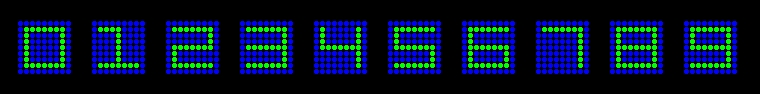
\includegraphics[width=0.99\textwidth]{pre_study_dataset}
    \caption[Straight Line Digits Dataset]{A novel dataset created to investigate the properties of modern deep learning architectures. The dataset consists of images of the numbers $0-9$, each image has a size of $9\times9$ pixels. The blue dots represent pixels with the value $0$, green dots represent pixels with the value $1$.}
    \figlbl{pre_study_dataset}
\end{figure}

The goal of this task is to predict the number (labels $0-9$) that is shown in the image.
This task is neither for humans nor deep learning architectures challenging.
However, it is simple enough to investigate the activations of neural networks and to search for net fragments.

The following example explains how net fragments could theoretically be built in this data set.
In total, the data set consists of $9$ basic lines, that can be composed to $10$ different digits.
A low-level net fragment could represent such a basic line and be composed to higher-level net fragments such as digits.
Figure \figref*{pre_study_components} visualizes these components (basic lines on the left, digits on the right).

\begin{figure}[h]
    \centering
    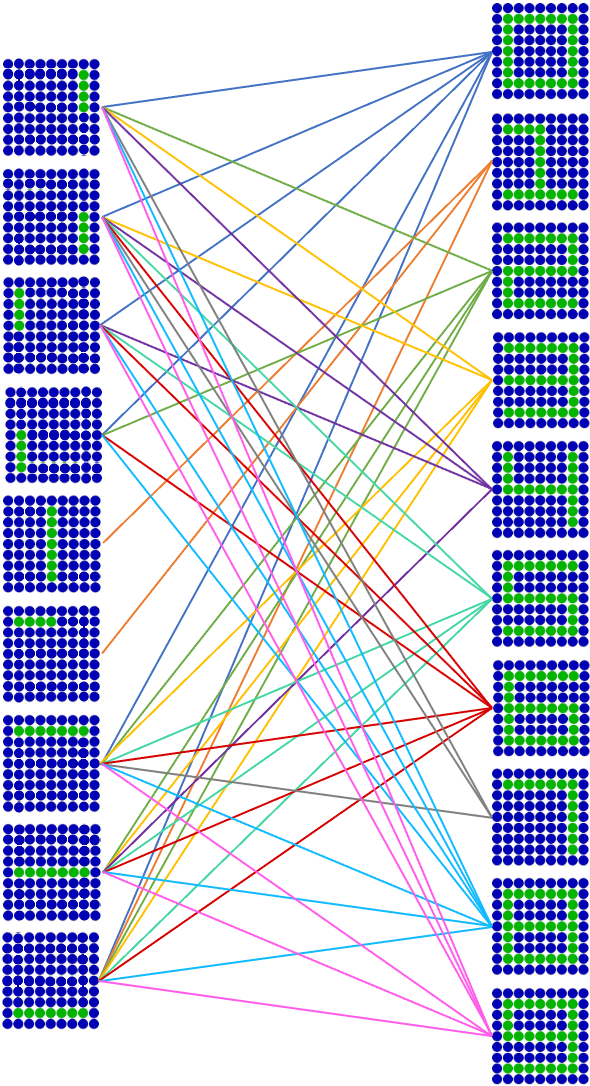
\includegraphics[width=0.99\textwidth]{pre_study_components}
    \caption[Line Types in Straight Line Digits Dataset]{A visualisation of all the lines (left) needed to compose the digits in the data set (right). The coloured lines in-between illustrate the relationship between the lines and the digits.}
    \figlbl{pre_study_components}
\end{figure}

Thereby, each low-level fragment can be part of one or multiple digits.
The composition can either take place across one or multiple layers.
The visualization in Figure \figref*{pre_study_components} can be interpreted as a composition across one layer, i.e. the low-level fragments are combined to high-level fragments within one step.

The composition can also take place across multiple layers. 
An exemplary composition of net fragments of the number $9$ across $4$ subsequent layers is shown in Figure \figref*{pre_study_composition}.
In this example, it is demonstrated that a fragment representing a digit can be composed of other fragments that also represent digits.
However, net fragments do not necessarily have to represent digits as shown in this example but can be a composition of multiple pixels without semantic.

\begin{figure}[h]
    \centering
    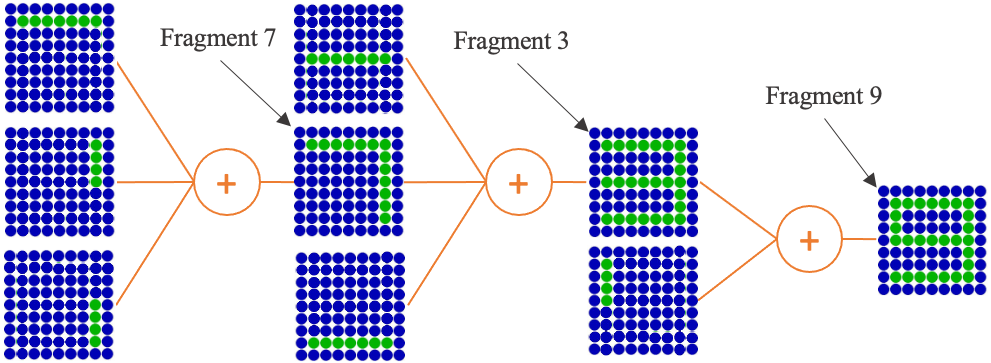
\includegraphics[width=0.99\textwidth]{pre_study_composition}
    \caption[Sample Net Fragment Composition]{A sample composition of the net fragment that could represent the digit $9$.}
    \figlbl{pre_study_composition}
\end{figure}

The fragments described so far are to be understood as an explanatory example.
A neural network might extract features in the first layers that do not correspond to vertical and horizontal lines and subsequently compose those features into more complex net fragments that are not as simple-to-interpret.
Meaning that looking for neurons of a (for us humans) simple to interpret meaning might be hard.
Regardless of what these net fragments represent, the network should have certain characteristics;
If a neuron or a group of neurons are part of a net fragment that represents a feature in the input, then these neuron(s) should be strongly active if the feature is present and not or only very weakly active if the feature is not present.
This leads to a sparse activation map and net fragments should only be active for digits with specific characteristics.
Furthermore, digits have common traits;
for example, the $7$ is contained in the $3$, the $3$ is contained in the $9$ and the $9$ is contained in the $8$.
The $1$, on the other hand, has nothing in common with the $4$, etc.
This means that at least one net fragment should be active for the $7$, $3$, $9$, and $8$ but not all net fragments that are composed to the digit $8$ should be active if the input depicts a $9$, $3$, or $7$.
The net fragments between the $1$ and $4$, on the other hand, should be completely different.
These properties should be visible in the activations of the network if it forms proper net fragments and are analysed in the following.

\section{Methods}\seclbl{pre_study_methods}
To investigate the emergence of net fragments, different deep learning models are trained.
The models are trained on a supervised classification task to predict the corresponding class of the images of the dataset shown in Figure \figref*{pre_study_dataset}.
The model's parameters are optimised by minimising the cross-entropy loss with the Adam optimizer \sidecite{Kingma2015AdamAM}.
The learning rate is $5 \cdot 10^{-4}$, the mini-batch size is $32$ samples and the model is trained for a total of $10$ epochs.

The models used have different feature extractors consisting of either convolutional (Conv.) layers (models no. $1$-$8$, no. $11$) or fully connected (FC) layers (models no. $10$) as shown in Table \tabref*{pre_study_models}.
Model no. $9$ has no feature extractor as the input images are so simple that they can be considered as features by themself, model no. $10$ uses a FC layer as feature extractor, and model no. $11$ has a Conv. layer with two hand-crafted kernels to extract horizontal and vertical lines as feature extractor.
After the feature extractor, all models have a similar ``head'' consisting of $2$ fully connected layers.
The feature extractor aims to extract certain features from the image, that are combined into higher-level net fragments in the first fully connected layer of the ``head'' and composed into predictions per class (i.e. net fragments corresponding to classes) in the last fully connected layer of the ``head''.
The first FC layer of the ``head'' consists of $12$ neurons.
The number of neurons was determined empirically by training various architectures and examining the number of active neurons.
It was found that there are always fewer than $12$ neurons active and that this capacity is therefore sufficient.
The last fully connected layer consists of $10$ neurons since this corresponds to the number of classes to predict.
The encoders of the models used are described in more detail in Table \tabref*{pre_study_models}.
The ``head'' is identical for all models and consists of a sequence of the following layers; FC ($12$ neurons) $\rightarrow$ ReLU $\rightarrow$ FC ($10$ neurons) $\rightarrow$ Softmax.

\begin{table}[h]
\newcolumntype{L}[1]{>{\raggedright\let\newline\\\arraybackslash\hspace{0pt}}m{#1}}
\newcolumntype{C}[1]{>{\centering\let\newline\\\arraybackslash\hspace{0pt}}m{#1}}
\newcolumntype{R}[1]{>{\raggedleft\let\newline\\\arraybackslash\hspace{0pt}}m{#1}}
    \tablbl{pre_study_models}
    \centering
	 \begin{tabular}{|l L{9cm}|} 
    	\hline
    	\textbf{No.} & \textbf{Encoder Description} \\
        \hline
		1 & Conv. Layer (kernel size=$3\times3$, channels=$2$) $\rightarrow$ ReLU $\rightarrow$ head \\ \hline
		2 & Conv. Layer (kernel size=$3\times3$, channels=$4$) $\rightarrow$ ReLU $\rightarrow$ head \\ \hline
		3 & Conv. Layer (kernel size=$5\times5$, channels=$2$) $\rightarrow$ ReLU $\rightarrow$ head \\ \hline
		4 & Conv. Layer (kernel size=$5\times5$, channels=$4$) $\rightarrow$ ReLU $\rightarrow$ head \\ \hline
		5 & Conv. Layer (kernel size=$3\times3$, channels=$2$) $\rightarrow$ ReLU $\rightarrow$ Conv. Layer (kernel size=$3\times3$, channels=$4$) $\rightarrow$ ReLU $\rightarrow$ head \\ \hline
		6 & Conv. Layer (kernel size=$3\times3$, channels=$4$) $\rightarrow$ ReLU $\rightarrow$ Conv. Layer (kernel size=$3\times3$, channels=$8$) $\rightarrow$ ReLU $\rightarrow$ head\\ \hline
		7 & Conv. Layer (kernel size=$3\times3$, channels=$2$) $\rightarrow$ ReLU $\rightarrow$ Max Pooling $\rightarrow$ Conv. Layer (kernel size=$3\times3$, channels=$4$) $\rightarrow$ ReLU $\rightarrow$ head\\ \hline
		8 & Conv. Layer (kernel size=$3\times3$, channels=$4$) $\rightarrow$ ReLU $\rightarrow$ Max Pooling $\rightarrow$ Conv. Layer (kernel size=$3\times3$, channels=$8$) $\rightarrow$ ReLU $\rightarrow$ head\\ \hline
		9 & head \\ \hline
		10 & FC ($9*9$ neurons) $\rightarrow$ ReLU $\rightarrow$ head \\ \hline
		11 & Hand Crafted Conv. Layer for vertical \& horizontal edge detection (kernel size=$3\times3$, channels=$2$) $\rightarrow$ ReLU $\rightarrow$ head \\
        \hline
    \end{tabular}
    \caption[Different Architectures for Preliminary Study]{A description of the different models used in the preliminary study.}
\end{table}

After each epoch, the model's weights are stored as well as the activations of each layer.
These vectors are visualized and investigated for net fragments.

Furthermore, the most relevant input features for a fully trained model are analysed.
This is done by freezing the model's parameters so that they cannot change.
Instead, an empty image is fed into the network and updated with backpropagation of error such that the probability for a given class is maximized.
This leads to an input image that has the highest probability to be predicted by the model as a specific class (e.g. generate the image that has the highest probability to be predicted as digit $3$ by the model).


\section{Results}\seclbl{pre_study_results}
All the models learn to classify these digits perfectly within a few epochs.
Interestingly, not only the accuracy reaches $100\%$ but some models also achieve a cross-entropy loss of $0.0$, meaning that they can find a global minimum.
However, the goal is not to achieve high accuracy but to exhibit net fragments.
It is not feasible to visualise all activations of all layers in this thesis.
Therefore, only the activations of the second last FC layer (i.e. the first FC layer of the ``head'') after the ReLU function are shown.
Since the last layer contains the net fragments that depict classes, this is the layer with the highest-level fragments.
Furthermore, it is the only layer that has a global view on the input, i.e. can access all the features extracted by the encoder\sidenote{convolutional layers only consider a local neighbourhood by sliding a kernel over the input (c.f. \secref{cnns})} (except for the encoder consisting of FC layers only).
Some higher-level net fragments should be visible in this layer, which are subsequently composed in the last layer to net fragments corresponding to classes.
Interested readers who want to investigate the activations from all layers, as well as the network weights by themselves, can view an interactive visualisation at \url{http://160.85.252.38:8501}.

\figref{pre_study_activations} shows the activations of the first fully connected layer in the ``head'' of the different models.
The FC layer has $12$ neurons whose activation is indicated along the vertical axis (per model), and the horizontal axis depicts the activation of the same neuron for the classes $0$-$9$.
For example, the circle in the top left corner indicates the activation of the first neuron for class $0$, the circle in the top right corner the activation of the first neuron for class $9$, and the circle in the bottom left corner the activation of the last neuron for class $0$.
Blue circles show activations that are exactly $0$, red circles are low activations $>0$, and green circles represent strong activations\sidenote{activations $<0$ do not exist because they are set to exactly $0$ by the ReLU function}.

It can be seen in the visualization that none of the models utilises all $12$ neurons and certain neurons are always inactive regardless of the class.
Also, no obvious net fragments can be identified;
Most neurons are always similarly strongly active regardless of the class.
If net fragments are formed, however, the neurons of a fragment would have to be strongly active in the presence of certain features and weakly active otherwise.
Such behaviour is not observable in these activations.

Furthermore, some digits are very similar and differ in only two pixels.
Some examples are the digit pairs $5$ and $6$, $8$ and $9$, $0$ and $8$, or $3$ and $9$.
However, when the activations of the corresponding classes are compared, it is obvious that almost always all activations change a little bit, and not one neuron is turned on or off depending on the presence of these two pixels.

\begin{figure}[h]
    \centering
    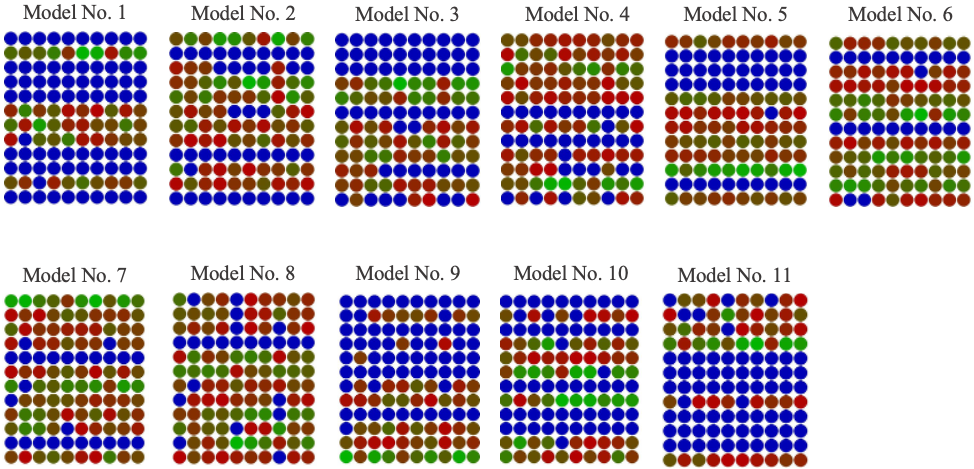
\includegraphics[width=0.99\textwidth]{pre_study_activations}
    \caption[Network Activations for Straight Line Digits Dataset]{The activations of the first fully connected layer in the ``head'' of the different networks. For each model, the activity of the $12$ neurons is shown for each class (activations along the vertical axis, classes along the horizontal axis). Red means low activation, green means high activation, blue means activation is off (i.e. $0$).}
    \figlbl{pre_study_activations}
\end{figure}

%It can also be observed that roughly the same neurons are always active.
%For different classes, however, these neurons do not switch on or off, but the strength of the activity changes.

\figref{pre_study_inputs_max} visualizes the input that maximizes the probability for each class.
It is obvious that all models focus on the wrong features and it can be assumed that these networks would not be robust to slight perturbations in the input.
This also indicates that net fragments are not present in current deep learning models (or at least not to the desirable extent);
if a class-level net fragment is composed of several lower-level net fragments, then some of these lower-level net fragments have to be active.
Since these lower-level net fragments represent specific input features, corresponding pixel constellations should be visible in this visualisation.
However, since these rather random-looking pixel combinations maximise the probability of predicting a specific class, this suggests that pixel combinations are not composed into hierarchically more complex net fragments.

\begin{figure}[h]
    \centering
    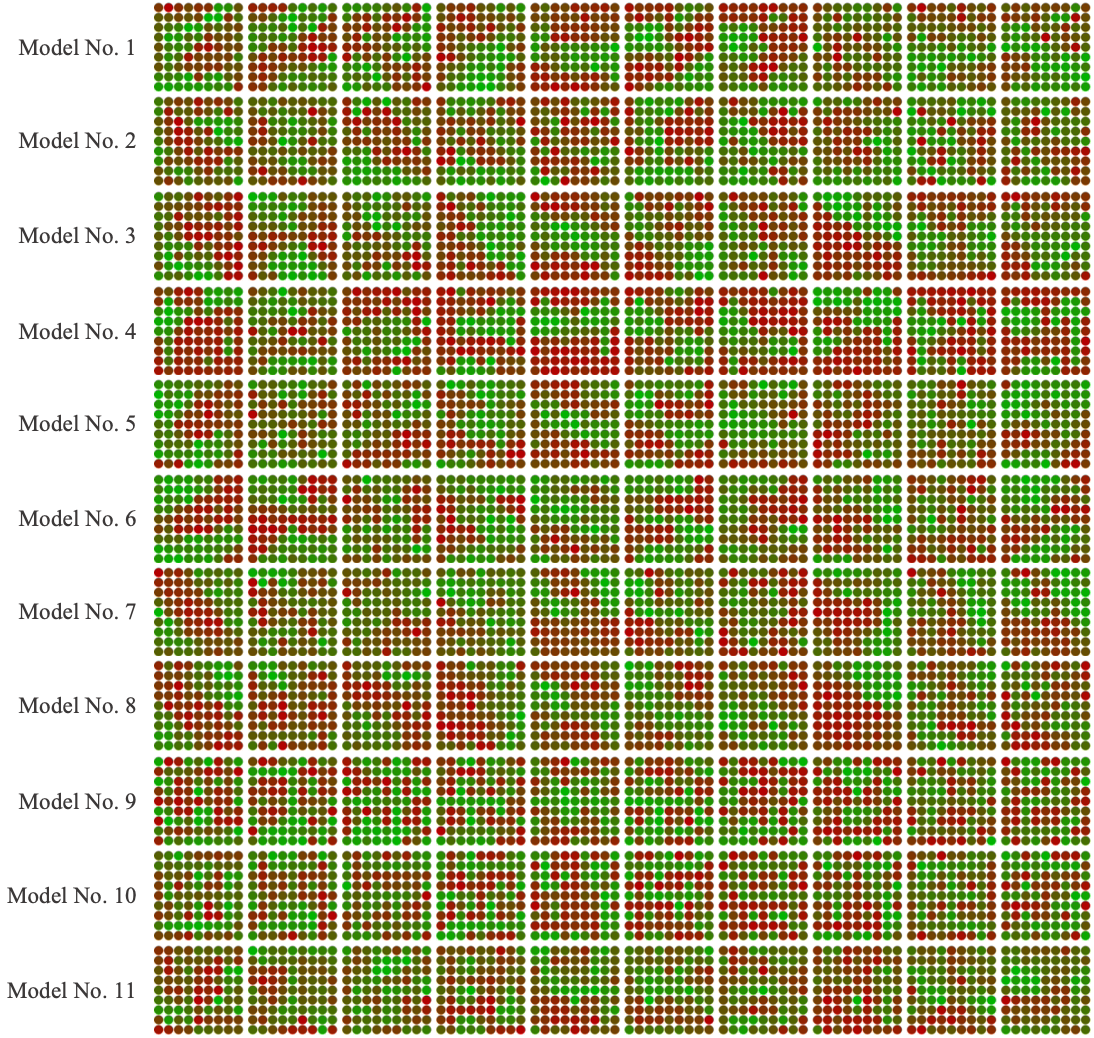
\includegraphics[width=0.99\textwidth]{pre_study_inputs_max}
    \caption[Inputs that Maximize the Class Output Probability]{The inputs that maximize the probability that the different models predict a specific class. For example, the image in the top left corner maximizes the probability that model number $1$ predicts that this is class $0$ (digit $0$).}
    \figlbl{pre_study_inputs_max}
\end{figure}


\section{Conclusion}\seclbl{pre_study_conclusion}
Different architectures have been trained on a very simple and therefore easily interpretable data set.
It was found that certain neurons are never active, while the active neurons usually remain active regardless of the class of the input data and only change their activity slightly.
Net fragments, on the other hand, rely on being strongly active when the corresponding feature they represent is present in the input and are weakly active or not active at all when it is not present.
Therefore, I argue that deep learning architectures do not comprise net fragments by default.

This assumption is further strengthened by the visualisation of the input that maximises the probability per class.
If a class is represented by a net fragment and this net fragment is composed of other net fragments, then some of these lower-level fragments would have to be active.
Such a set of low-level net fragments can directly be mapped to a set of pixels that has to be active.
However, since the input does not contain a meaningful (sub-) set of active pixels, it can be assumed that these lower-level fragments are either not present or at least do not represent any meaningful features.


TODO: Autoencoder, Sparse-Autoencoder in Pre-Study